% ===========================================================================
% Appendix B: simulation tables referred to from §4 (simulation.tex).
% Generated files under paper/sim/; see simulation.tex for the pipeline.
% ===========================================================================

The tables below are the ones \S\ref{sec:sim} summarises.
\texttt{libqueuingsim} is an event-driven simulator in Rust. The
synthetic checks use $a=2\cdot10^{-5}$, $b=2\cdot10^{-9}$,
$\omega=2\cdot10^{-4}$ and $\beta=2\cdot10^{-9}$ seconds per token
unless a caption says otherwise; the replays of production sessions
(Tables~\ref{tab:sim-trace}, \ref{tab:sim-trace-price}
and~\ref{tab:sim-trace-split}) use the cost model calibrated on the
testbed (\S\ref{sec:exp-testbed}). Every number is generated by the
simulator from fixed seeds and is a property of the simulated model,
not a measurement; the best value in each comparison is in bold.

% Generated by `cargo run --release --example paper_tables` in
% libqueuingsim/. Do not edit by hand.
\begin{table}[t]
\caption{Simulation under each proposition's assumptions (in-model). M/M/1: $\mu=10$. PK: $\rho=0.7$. Cache: $\lambda=1.8$. SF/OPT: worst of 9000 instances with equal $p_i$. $\pm$ is a 95\,\% batch-means half-width. Times in seconds.}
\label{tab:sim-inmodel}
\centering\small
\begin{tabular}{@{}l@{\hspace{4pt}}lcc@{}}
\toprule
Quantity & Result & Theory & Simulated \\
\midrule
M/M/1 $W$, $\lambda=9$ & \S\ref{sec:intro} & 1.000 & $1.012 \pm 0.024$ \\
PK $W_q$, workload B & Thm.~\ref{thm:pk} & 4.002 & $3.960 \pm 0.052$ \\
$W_q^B/W_q^A$, $\rho=0.6$ & Prop.~\ref{prop:pk} & 3.43 & 3.42 \\
$\rho$ at $p=0.8$ & Prop.~\ref{prop:cache} & 0.252 & 0.253 \\
$W_q$ / M/M/1, $\mathrm{CV}^2{=}15.3$ & Eq.~\eqref{eq:cv2} & 8.15 & 8.10 \\
max SF/OPT & Prop.~\ref{prop:evict} & $\le 2$ & 1.791 \\
\bottomrule
\end{tabular}
\end{table}

% Generated by `cargo run --release --example paper_tables` in
% libqueuingsim/. Do not edit by hand.
\begin{table}[t]
\caption{Batching server under its assumptions (in-model): mean number of turns at the replica, $L=\lambda R$. Rows 1--4: Poisson turns at $\rho=0.7$, work deterministic or hit/miss ($0.05$\,s w.p.\ $0.8$, else $0.5$\,s; both mean $0.14$\,s); PS theory $\rho/(1-\rho)$, FIFO theory $\lambda W_q+\rho$. Rows 5--6: sessions arrive Poisson, each turn is followed by a tool call (mean 2\,s, $\mathrm{CV}^2=4$) and another turn w.p.\ $0.8$; theory $\sum_n n\pi(n)$ at $\lambda=\Lambda/(1-p)$ ($\rho=0.7$ for $\phi\equiv 1$, $\rho=3$ for $\phi(n)=n/(1+\beta(n-1))$). Row 7: rise of $L$ at a PS server when a fraction $\delta$ of turns becomes misses, hit rate $0.8$, $\rho=0.6$, against $[\lambda\delta\Phi_{\mathrm{PS}},\ \tfrac{C-\rho}{C-\rho'}\lambda\delta\Phi_{\mathrm{PS}}]$. Rows 8--9: the same misses on the two-resource replica (prefill FIFO in the compute left by a decode batch of $0.1$\,s per turn, mean availability $\bar r=0.96$): rise of the number in the prefill stage $L_P=\lambda\,\mathrm{TTFT}$ against the FIFO bracket at service $P/\bar r$, and of the number in the decode stage $L_D$, whose demand does not depend on hit or miss. $\pm$ is a 95\,\% batch-means half-width.}
\label{tab:sim-ps}
\centering\small\setlength{\tabcolsep}{3pt}
\begin{tabular}{@{}l@{\hspace{4pt}}lcc@{}}
\toprule
Quantity & Result & Theory & Simulated \\
\midrule
PS, D & \S\ref{sec:batch} & 2.333 & $2.338 \pm 0.021$ \\
PS, hit/miss & \S\ref{sec:batch} & 2.333 & $2.348 \pm 0.044$ \\
FIFO, D & Eq.~\eqref{eq:pk} & 1.517 & $1.519 \pm 0.011$ \\
FIFO, hit/miss & Eq.~\eqref{eq:pk} & 2.867 & $2.880 \pm 0.051$ \\
Loop, $\phi\equiv1$ & \S\ref{sec:sessions} & 2.33 & $2.36 \pm 0.07$ \\
Loop, sat.\ $\phi$ ($\beta{=}0.25$) & \S\ref{sec:sessions} & 12.00 & $12.32 \pm 0.39$ \\
PS $\Delta L$, $\delta{=}0.05$ & Prop.~\ref{prop:decode} & $[0.60,0.79]$ & $0.775 \pm 0.018$ \\
2-stage $\Delta L_P$, $\delta{=}0.05$ & Prop.~\ref{prop:price} & $[0.81,1.11]$ & $1.068 \pm 0.029$ \\
2-stage $\Delta L_D$, $\delta{=}0.05$ & Prop.~\ref{prop:decode} & 0 & $-0.000 \pm 0.000$ \\
\bottomrule
\end{tabular}
\end{table}

% Generated by `uv run python -m report.paper_tables` in
% validation/. Do not edit by hand.
\begin{table}[htbp]
\caption{Batch cap $B=8$: exact limited PS (at most $B$ turns share $\phi(n)=n/(1+0.1(n-1))$, FIFO beyond) against PS with $\phi$ flattened at $B$, the model's approximation. Poisson turns, work of mean 1 with the given law ($\mathrm{CV}^2$ in brackets), load $u=\rho/\phi(B)$. Mean number at the replica; last column: relative error of the approximation for LPS, in \%. Mean response time has the same relative error (Little).}
\label{tab:sim-lps}
\centering\small\setlength{\tabcolsep}{3pt}
\begin{tabular}{@{}lccccc@{}}
\toprule
Work & $u$ & Formula & PS & LPS & Err. \\
\midrule
D (0) & 0.5 & 3.10 & $3.10 \pm 0.00$ & $3.08 \pm 0.00$ & $-1$ \\
D (0) & 0.8 & 7.33 & $7.33 \pm 0.06$ & $6.60 \pm 0.03$ & $-10$ \\
D (0) & 0.9 & 12.67 & $12.81 \pm 0.44$ & $9.90 \pm 0.22$ & $-22$ \\
Exp (1) & 0.5 & 3.10 & $3.11 \pm 0.01$ & $3.11 \pm 0.01$ & $+0$ \\
Exp (1) & 0.8 & 7.33 & $7.38 \pm 0.11$ & $7.38 \pm 0.11$ & $+1$ \\
Exp (1) & 0.9 & 12.67 & $12.73 \pm 0.52$ & $12.72 \pm 0.52$ & $+0$ \\
H2 (4) & 0.5 & 3.10 & $3.09 \pm 0.03$ & $3.12 \pm 0.03$ & $+1$ \\
H2 (4) & 0.8 & 7.33 & $7.29 \pm 0.18$ & $9.14 \pm 0.44$ & $+25$ \\
H2 (4) & 0.9 & 12.67 & $12.57 \pm 0.72$ & $20.31 \pm 1.87$ & $+60$ \\
\bottomrule
\end{tabular}
\end{table}


\begin{figure}[t]
\centering
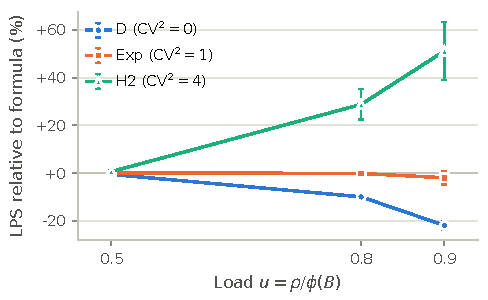
\includegraphics[width=\columnwidth]{sim/fig-lps}
\caption{Error of the saturating-$\varphi$ formula against an exact
batch cap ($B=8$) as a function of load, one line per work law. The
sign follows the work $\mathrm{CV}^2$. Synthetic, uncalibrated.}
\label{fig:sim-lps}
\end{figure}

% Generated by `cargo run --release --example paper_tables` in
% libqueuingsim/. Do not edit by hand.
\begin{table}[t]
\caption{Offline eviction: cost relative to the exact optimum of \eqref{eq:evict} with costs $p_ic_i^2$, over 3000 random instances per row (12 programs, $c_i\in\{1,\dots,200\}$, $\Delta C$ a random 10--60\,\% of the total).}
\label{tab:sim-evict}
\centering\small
\begin{tabular}{@{}lcccc@{}}
\toprule
Resume model & \multicolumn{2}{c}{SF mean / max} & \multicolumn{2}{c}{Density mean / max} \\
\midrule
equal $p_i$ & 1.108 & 1.67 & 1.108 & 1.67 \\
$p_i\sim U[0.05,1]$ & 1.902 & 10.05 & 1.136 & 2.86 \\
$p_i$ falls with $c_i$ & 2.037 & 8.60 & 1.146 & 2.67 \\
\bottomrule
\end{tabular}
\end{table}


\begin{figure}[t]
\centering
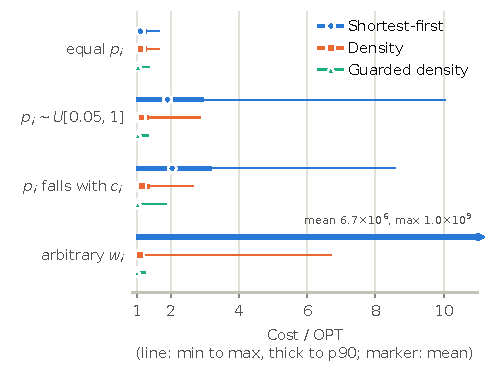
\includegraphics[width=\columnwidth]{sim/fig-evict-offline}
\caption{Offline eviction cost relative to the exact optimum by rule
and regime (mean, with the worst instance marked). Synthetic,
uncalibrated.}
\label{fig:sim-evict}
\end{figure}

% Generated by `uv run python -m report.paper_tables` in
% validation/. Do not edit by hand.
\begin{table}[htbp]
\caption{Eviction with open sessions on a replica with the vLLM~v1 engine's rules (those of Table~\ref{tab:sim-trace}) and the testbed's cost model. Sessions arrive Poisson at rate $\Lambda$ (per s): half agents ($p_i=0.95$, 4--8k initial tokens, tool calls Exp(6\,s)), half one-shot documents ($p_i=0.3$, 15--30k tokens, think time Exp(2\,s)); 600k-token KV, batch cap 8, at most 24 live sessions. Every policy evicts 16-token blocks from the tail of a context, sessions in a tool call before waiting ones (except LRU), and drops a finished session's blocks; rows marked $^*$ keep them, as vLLM's engine does, which cannot tell a finished session from one in a tool call. Throughput (turns/s), follow-up hit rate (the whole reusable prefix reused), mean and p99 time to first token (s), mean turn response (s; its half-width is in the data file), and the number of the 20 seeds that thrashed (follow-up turns reusing less than half of their reusable prefix); $\pm$ is a 95\,\% half-width over seeds; the best throughput, hit rate, TTFT and p99 per load in bold. Priced: $p_i\Phi_i/c_i$ with the FIFO price of Prop.~\ref{prop:price} from online estimates at the engine; Priced/$\tau$: per byte-second, $p_i\Phi_i/(c_i\tau_i)$ (the threshold rule of \S\ref{sec:evict}); Blocks: the same price of the tail block. The priced rules take $p_i$ and $\tau_i$ from the generating class (an oracle); the fixed keys see neither.}
\label{tab:sim-evict-dyn}
\centering\small\setlength{\tabcolsep}{2pt}
\begin{tabular}{@{}clcccccc@{}}
\toprule
$\Lambda$ & Policy & $X$ & Hit & TTFT & p99 & $R$ & Thr. \\
\midrule
0.03 & SF & \textbf{0.29} & \textbf{1.00} & $\mathbf{2.22 \pm 0.15}$ & \textbf{16.8} & 20.2 & 0 \\
0.03 & Density & \textbf{0.29} & \textbf{1.00} & $\mathbf{2.22 \pm 0.15}$ & \textbf{16.8} & 20.2 & 0 \\
0.03 & Priced & \textbf{0.29} & \textbf{1.00} & $\mathbf{2.22 \pm 0.15}$ & \textbf{16.8} & 20.2 & 0 \\
0.03 & Priced/$\tau$ & \textbf{0.29} & \textbf{1.00} & $\mathbf{2.22 \pm 0.15}$ & \textbf{16.8} & 20.2 & 0 \\
0.03 & Blocks & \textbf{0.29} & \textbf{1.00} & $\mathbf{2.22 \pm 0.15}$ & \textbf{16.8} & 20.2 & 0 \\
0.03 & LRU & \textbf{0.29} & \textbf{1.00} & $\mathbf{2.22 \pm 0.15}$ & \textbf{16.8} & 20.2 & 0 \\
0.03 & LRU$^*$ & \textbf{0.29} & \textbf{1.00} & $\mathbf{2.22 \pm 0.15}$ & \textbf{16.8} & 20.2 & 0 \\
0.03 & Priced/$\tau$$^*$ & \textbf{0.29} & 0.59 & $4.80 \pm 0.50$ & 29.3 & 23.6 & 0 \\
0.05 & SF & \textbf{0.38} & \textbf{0.83} & $34.45 \pm 1.01$ & 70.4 & 53.4 & 0 \\
0.05 & Density & \textbf{0.38} & \textbf{0.83} & $\mathbf{34.39 \pm 1.01}$ & \textbf{69.6} & 53.4 & 0 \\
0.05 & Priced & \textbf{0.38} & \textbf{0.83} & $34.48 \pm 0.99$ & 70.7 & 53.5 & 0 \\
0.05 & Priced/$\tau$ & \textbf{0.38} & \textbf{0.83} & $34.43 \pm 1.01$ & 70.4 & 53.4 & 0 \\
0.05 & Blocks & \textbf{0.38} & \textbf{0.83} & $34.46 \pm 1.00$ & 70.6 & 53.5 & 0 \\
0.05 & LRU & 0.27 & 0.75 & $56.41 \pm 1.76$ & 226.2 & 77.3 & 0 \\
0.05 & LRU$^*$ & 0.24 & 0.70 & $66.89 \pm 2.39$ & 240.9 & 88.2 & 0 \\
0.05 & Priced/$\tau$$^*$ & 0.35 & 0.45 & $41.73 \pm 0.68$ & 71.8 & 61.6 & 0 \\
\bottomrule
\end{tabular}
\end{table}

% Generated by `uv run python -m report.paper_tables` in
% validation/. Do not edit by hand.
\begin{table}[htbp]
\caption{Admission-cap sweep on the vLLM-rule replica: the scenario of Table~\ref{tab:sim-evict-dyn} with at most 16, 24 or 32 live sessions; later arrivals wait in an entry queue. Throughput (turns/s), follow-up hit rate, mean and p99 time to first token (s), mean turn response (s), mean entry-queue wait of a new session (s), and the number of the 20 seeds that thrashed. Means over seeds; the best throughput, hit rate, TTFT and p99 per ($\Lambda$, cap) in bold. The 95\,\% half-widths over seeds are the whiskers of Figure~\ref{fig:sim-admission}; Table~\ref{tab:sim-evict-dyn} states them for the rows it shares. An entry wait of hundreds of seconds means the replica does not carry the offered turn rate and the entry queue grows over the run; such values depend on the horizon (20\,000\,s). Every policy drops a finished session's blocks.}
\label{tab:sim-admission}
\centering\small\setlength{\tabcolsep}{2pt}
\begin{tabular}{@{}ccl@{\hspace{3pt}}cccccccc@{}}
\toprule
$\Lambda$ & Cap & Policy & $X$ & Hit & TTFT & p99 & $R$ & Entry & Thr. \\
\midrule
0.03 & 16 & SF & \textbf{0.29} & \textbf{1.00} & \textbf{2.21} & \textbf{16.5} & 20.20 & 0.1 & 0 \\
0.03 & 16 & Density & \textbf{0.29} & \textbf{1.00} & \textbf{2.21} & \textbf{16.5} & 20.20 & 0.1 & 0 \\
0.03 & 16 & Priced/$\tau$ & \textbf{0.29} & \textbf{1.00} & \textbf{2.21} & \textbf{16.5} & 20.20 & 0.1 & 0 \\
0.05 & 16 & SF & \textbf{0.41} & \textbf{1.00} & \textbf{14.54} & \textbf{33.5} & 32.89 & 1297.7 & 0 \\
0.05 & 16 & Density & \textbf{0.41} & \textbf{1.00} & \textbf{14.54} & \textbf{33.5} & 32.89 & 1297.7 & 0 \\
0.05 & 16 & Priced/$\tau$ & \textbf{0.41} & \textbf{1.00} & \textbf{14.54} & \textbf{33.5} & 32.89 & 1297.7 & 0 \\
0.03 & 24 & SF & \textbf{0.29} & \textbf{1.00} & \textbf{2.22} & \textbf{16.8} & 20.21 & 0.0 & 0 \\
0.03 & 24 & Density & \textbf{0.29} & \textbf{1.00} & \textbf{2.22} & \textbf{16.8} & 20.21 & 0.0 & 0 \\
0.03 & 24 & Priced/$\tau$ & \textbf{0.29} & \textbf{1.00} & \textbf{2.22} & \textbf{16.8} & 20.21 & 0.0 & 0 \\
0.05 & 24 & SF & \textbf{0.38} & \textbf{0.83} & 34.45 & 70.4 & 53.44 & 1407.5 & 0 \\
0.05 & 24 & Density & \textbf{0.38} & \textbf{0.83} & \textbf{34.39} & \textbf{69.6} & 53.38 & 1407.3 & 0 \\
0.05 & 24 & Priced/$\tau$ & \textbf{0.38} & \textbf{0.83} & 34.43 & 70.4 & 53.42 & 1408.4 & 0 \\
0.03 & 32 & SF & \textbf{0.29} & \textbf{1.00} & \textbf{2.22} & \textbf{16.8} & 20.21 & 0.0 & 0 \\
0.03 & 32 & Density & \textbf{0.29} & \textbf{1.00} & \textbf{2.22} & \textbf{16.8} & 20.21 & 0.0 & 0 \\
0.03 & 32 & Priced/$\tau$ & \textbf{0.29} & \textbf{1.00} & \textbf{2.22} & \textbf{16.8} & 20.21 & 0.0 & 0 \\
0.05 & 32 & SF & \textbf{0.32} & \textbf{0.57} & \textbf{64.01} & 144.5 & 84.49 & 1657.0 & 0 \\
0.05 & 32 & Density & \textbf{0.32} & \textbf{0.57} & 64.18 & \textbf{143.9} & 84.69 & 1659.3 & 0 \\
0.05 & 32 & Priced/$\tau$ & \textbf{0.32} & \textbf{0.57} & 64.10 & 145.1 & 84.58 & 1661.9 & 0 \\
\bottomrule
\end{tabular}
\end{table}


\begin{figure}[t]
\centering
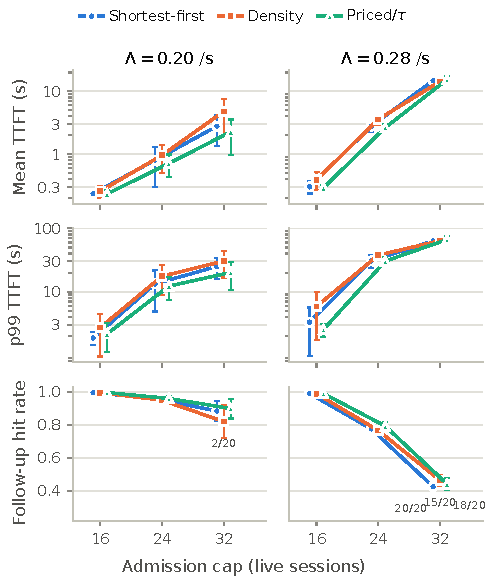
\includegraphics[width=\columnwidth]{sim/fig-admission}
\caption{Admission-cap sweep on the two-resource replica: mean and p99
time to first token (log scale) and hit rate by cap and eviction rule at
two session arrival rates; annotations give the number of seeds (of 20)
that thrashed. Synthetic, uncalibrated.}
\label{fig:sim-admission}
\end{figure}

% Generated by `uv run python -m report.paper_tables` in
% validation/. Do not edit by hand.
\begin{table}[htbp]
\caption{Placement over 4 replicas with half of the new programs placed on replica~0 (the affinity node), follow-up turns of 5--15k-token contexts, state moved over one shared link of bandwidth $B$ (tokens/s) when that is cheaper than recomputing it. $x$: mean move cost over mean service; $\rho^*=x/(1+x)$, the inversion utilisation of Eq.~\eqref{eq:rhostar} for one node and an idle alternative; Inv.: the lowest program rate (per s, swept in steps of 0.05) at which always moving to the least-loaded replica beats affinity in mean turn response beyond both confidence intervals; $\rho_0$: utilisation of the affinity node at that rate; $\rho_L$: utilisation of the shared link under always-move there; mean turn response (s) of affinity, always-move and the lookahead rule of Eq.~\eqref{eq:lookahead}. The idle alternative gives the earliest inversion, so $\rho^*$ is a lower bound for any real alternative.}
\label{tab:sim-inversion}
\centering\scriptsize\setlength{\tabcolsep}{2pt}
\begin{tabular}{@{}ccccccccc@{}}
\toprule
$B$ & $x$ & $\rho^*$ & Inv. & $\rho_0$ & $\rho_L$ & Affinity & Move & Lookahead \\
\midrule
20000k & 0.01 & 0.01 & $\le 0.20$ & 0.13 & 0.00 & 0.082 & 0.072 & 0.072 \\
2000k & 0.08 & 0.08 & $\le 0.20$ & 0.13 & 0.00 & 0.082 & 0.074 & 0.072 \\
500k & 0.34 & 0.25 & 0.40 & 0.26 & 0.05 & 0.096 & 0.090 & 0.076 \\
125k & 1.32 & 0.57 & 1.60 & 0.98 & 0.96 & 4.621 & 0.983 & 0.120 \\
\bottomrule
\end{tabular}
\end{table}

% Generated by `cargo run --release --example paper_tables` in
% libqueuingsim/. Do not edit by hand.
\begin{table}[t]
\caption{A FIFO prefill queue fed by $N$ live sessions, each thinking for an exponential time of mean $Z$ (s) and then submitting a turn of exponential work with mean $1$\,s, with $Z$ chosen so that the server utilisation is $\rho=0.6$ for every $N$. Mean wait in queue (s): exact finite-source value (M/M/1//$N$), simulated (95\,\% batch-means half-width), and the open M/M/1 wait $\rho/(\mu(1-\rho))$ that the PK formula gives from the measured rate and moments; last column their ratio.}
\label{tab:sim-finite}
\centering\small\setlength{\tabcolsep}{3pt}
\begin{tabular}{@{}cccccc@{}}
\toprule
$N$ & $Z$ & Exact & Simulated & Open & Open/Exact \\
\midrule
2 & 2.0 & 0.333 & $0.336 \pm 0.007$ & 1.500 & 4.50 \\
4 & 5.0 & 0.646 & $0.650 \pm 0.013$ & 1.500 & 2.32 \\
8 & 11.4 & 0.914 & $0.902 \pm 0.015$ & 1.500 & 1.64 \\
16 & 24.5 & 1.126 & $1.123 \pm 0.019$ & 1.500 & 1.33 \\
64 & 104.3 & 1.375 & $1.383 \pm 0.033$ & 1.500 & 1.09 \\
\bottomrule
\end{tabular}
\end{table}

% Generated by `cargo run --release --example paper_tables` in
% libqueuingsim/. Do not edit by hand.
\begin{table}[t]
\caption{Forced misses on the replayed production sessions with no pool limit (open, Poisson sessions at rate $\Lambda$ per s, at most 24 live, 60000\,s of measurement after 6000\,s of warm-up: the configuration of the first rows of Table~\ref{tab:sim-trace}). A share $\delta$ of follow-up turns whose context is resident is forced to miss. $\bar N$, $\bar N'$: mean live sessions in the baseline and in the forced run; $\rho$: prefill load of the baseline; $\rho'$: the load the added work implies; $L_P$: baseline mean number in the prefill stage; $\Delta L_P$: its rise in the forced run, mean and 95\,\% half-width over 10 seeds; $[\mathrm{lo},\mathrm{hi}]$: the bracket of Proposition~\ref{prop:price} from the baseline's measured $\lambda$, $\rho$, $W$ and each forced turn's own $S^{\mathrm{hit}}$, $S^{\mathrm{miss}}$ ($\rho'\ge1$: the open queue would be unstable); Finite: the rise of Proposition~\ref{prop:finite}'s recursion for the added mean work, with $N=\bar N$ rounded and the corpus mean think time; Fin.: that finite-source rise; cap: $\bar N'-L_P$.}
\label{tab:sim-trace-price}
\centering\scriptsize\setlength{\tabcolsep}{2pt}
\begin{tabular}{@{}cccccccccccc@{}}
\toprule
$\Lambda$ & $\delta$ & $\bar N$ & $\bar N'$ & $\rho$ & $\rho'$ & $L_P$ & $\Delta L_P$ & lo & hi & Fin. & cap \\
\midrule
0.005 & 0.01 & 4.7 & 6.2 & 0.25 & 0.39 & 0.7 & $1.5 \pm 1.2$ & 11.6 & 16.6 & 0.3 & 5.5 \\
0.005 & 0.03 & 4.7 & 8.0 & 0.25 & 0.58 & 0.7 & $3.3 \pm 1.3$ & 12.7 & 25.1 & 0.7 & 7.3 \\
0.005 & 0.10 & 4.7 & 18.5 & 0.25 & 0.97 & 0.7 & $14.4 \pm 2.0$ & 20.4 & $\rho'\ge1$ & 1.4 & 17.8 \\
0.010 & 0.01 & 12.1 & 18.1 & 0.51 & 0.78 & 3.3 & $6.6 \pm 1.4$ & 54.0 & 136.6 & 1.7 & 14.8 \\
0.010 & 0.03 & 12.1 & 22.7 & 0.51 & 1.03 & 3.3 & $12.5 \pm 0.8$ & 72.0 & $\rho'\ge1$ & 3.3 & 19.4 \\
0.010 & 0.10 & 12.1 & 23.7 & 0.51 & 1.28 & 3.3 & $16.8 \pm 0.7$ & 79.5 & $\rho'\ge1$ & 4.5 & 20.5 \\
\bottomrule
\end{tabular}
\end{table}

% Generated by `cargo run --release --example paper_tables` in
% libqueuingsim/. Do not edit by hand.
\begin{table}[t]
\caption{Replayed production sessions on the two-resource replica: 761 Claude Code sessions (26395 turns, mean final context 391k tokens, mean think time 23\,s) from the corpus of \S\ref{sec:exp-traces}, arriving Poisson at rate $\Lambda$ (per s), each played turn by turn; cost model with $K_c=a/b=50$k tokens, batch cap 8, eviction by price per byte-second, at most Cap live sessions (the rest wait to enter). Follow-up hit rate; the share of $\mathrm{Var}[S]$ of follow-up prefill work due to the hit/miss mixture (the rest is the spread of the appends) and the $\mathrm{CV}^2$ of that work; observed mean prefill wait $W_q$ and the PK wait from the measured $\lambda$, $\E[S]$, $\E[S^2]$ (s); mean TTFT (s). Entry waits of sessions held by the cap are in the data file. $\pm$ is a 95\,\% half-width over 5 seeds.}
\label{tab:sim-trace}
\centering\small\setlength{\tabcolsep}{2pt}
\begin{tabular}{@{}ccccccccc@{}}
\toprule
$\Lambda$ & Pool & Cap & Hit & Mix & $\mathrm{{CV}}^2$ & $W_q$ & PK & TTFT \\
\midrule
0.005 & $\infty$ & 24 & $1.00 \pm 0.00$ & 0.00 & 43.4 & 3 & 12 & 5 \\
0.005 & 4M & 8 & $0.92 \pm 0.10$ & 0.38 & 53.5 & 71 & 664 & 83 \\
0.005 & 4M & 16 & $0.74 \pm 0.35$ & 0.29 & 28.6 & 192 & 1954 & 206 \\
0.005 & 2M & 4 & $0.80 \pm 0.13$ & 0.59 & 8.1 & 66 & 703 & 91 \\
0.005 & 2M & 8 & $0.25 \pm 0.25$ & 0.18 & 1.9 & 302 & 5946 & 349 \\
0.005 & 1M & 2 & $0.86 \pm 0.09$ & 0.75 & 9.3 & 10 & 81 & 24 \\
0.005 & 1M & 4 & $0.51 \pm 0.12$ & 0.44 & 2.5 & 79 & 669 & 111 \\
0.010 & $\infty$ & 24 & $1.00 \pm 0.00$ & 0.00 & 35.2 & 9 & 36 & 11 \\
0.010 & 4M & 8 & $0.84 \pm 0.11$ & 0.41 & 22.1 & 133 & 1546 & 154 \\
0.010 & 4M & 16 & $0.28 \pm 0.20$ & 0.17 & 2.3 & 540 & 4093 & 578 \\
0.010 & 2M & 4 & $0.80 \pm 0.16$ & 0.58 & 9.7 & 66 & 706 & 92 \\
0.010 & 2M & 8 & $0.21 \pm 0.19$ & 0.16 & 1.7 & 315 & 5344 & 363 \\
0.010 & 1M & 2 & $0.86 \pm 0.09$ & 0.75 & 9.3 & 10 & 81 & 24 \\
0.010 & 1M & 4 & $0.50 \pm 0.11$ & 0.43 & 2.4 & 81 & 701 & 113 \\
\bottomrule
\end{tabular}
\end{table}


% Generated by `cargo run --release --example paper_tables` in
% libqueuingsim/. Do not edit by hand.
\begin{table}[t]
\caption{Sensitivity of the open-pool replay ($\Lambda=0.005$, no pool limit) to the rule that starts a new session at a gap longer than the threshold: sessions in the corpus, mean turns and mean think time (s) per session, then mean live sessions, throughput (turns/s), follow-up prefill-work $\mathrm{CV}^2$, load, observed and PK prefill wait (s) and mean TTFT (s).}
\label{tab:sim-trace-split}
\centering\scriptsize\setlength{\tabcolsep}{2pt}
\begin{tabular}{@{}lcccccccccc@{}}
\toprule
Split & Sessions & Turns & Think & $\bar N$ & $X$ & $\mathrm{{CV}}^2$ & $\rho$ & $W_q$ & PK & TTFT \\
\midrule
10 min & 761 & 34.7 & 23 & 4.7 & 0.155 & 43.4 & 0.25 & 3 & 12 & 5 \\
30 min & 451 & 58.6 & 36 & 11.5 & 0.273 & 30.2 & 0.33 & 3 & 13 & 4 \\
\bottomrule
\end{tabular}
\end{table}

